\documentclass{standalone}

\usepackage{tikz}
\usepackage{circuitikz}

\tikzset{block/.style = {draw, fill=white, very thick, rectangle, minimum height=1cm, minimum width=2cm},
         lblock/.style={draw,fill=white,very thick, rectangle, minimum height=3cm, minimum width=1cm},
         sum/.style= {draw, fill=white, very thick, circle, node distance=0.5cm}}

         
\begin{document}
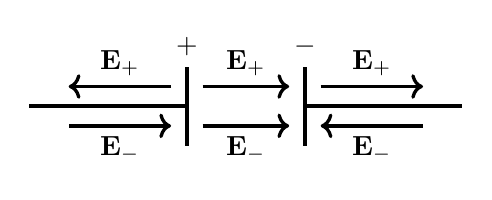
\begin{tikzpicture}[scale=2]
    \draw[-,very thick](-0.75,0)--(0.25,0);
    \draw[-,ultra thick](0.25,-0.25)--(0.25,0.25)node[above]{$+$};
    \draw[-, very thick](1,0)--(2,0);
    \draw[-,ultra thick](1,-0.25)--(1,0.25)node[above]{$-$};

    \draw[->,very thick](0.35,0.125)--(0.9,0.125)node[midway,above]{$\mathbf{E}_+$};
    \draw[->,very thick](1.1,0.125)--(1.75,0.125)node[midway,above]{$\mathbf{E}_+$};
    \draw[->,very thick](0.15,0.125)--(-0.5,0.125)node[midway,above]{$\mathbf{E}_+$};
    \draw[->,very thick](0.35,-0.125)--(0.9,-0.125)node[midway,below]{$\mathbf{E}_-$};
    \draw[<-,very thick](1.1,-0.125)--(1.75,-0.125)node[midway,below]{$\mathbf{E}_-$};
    \draw[<-,very thick](0.15,-0.125)--(-0.5,-0.125)node[midway,below]{$\mathbf{E}_-$};
\end{tikzpicture}
\end{document}